\documentclass{standalone}
\begin{document}
	\subsection{Expert Evaluation}
	
	Another measure for the pipeline performances was a blind evaluation. In collaboration with the Department of Diagnostic and Preventive Medicine of the Policlinico Sant'Orsola - Malpighi, $3$ experts with at least $2$ years of experience have compared the pipeline segmentation and the reference labels (Annotation) provided within the dataset (obtained by semi-automatic technique). 

	To perform the evaluation, I have randomly selected $10$ patients from the three datasets and organized the scans as follows:
	For each patient I have displayed, slice by slice, two images: the scans with the pipeline segmentation (the one to test), and the semi-automatic labels provided within the dataset (control) as in. \figurename\,\ref{fig:Blind}.
	
	\begin{figure}[h!]
		\centering
		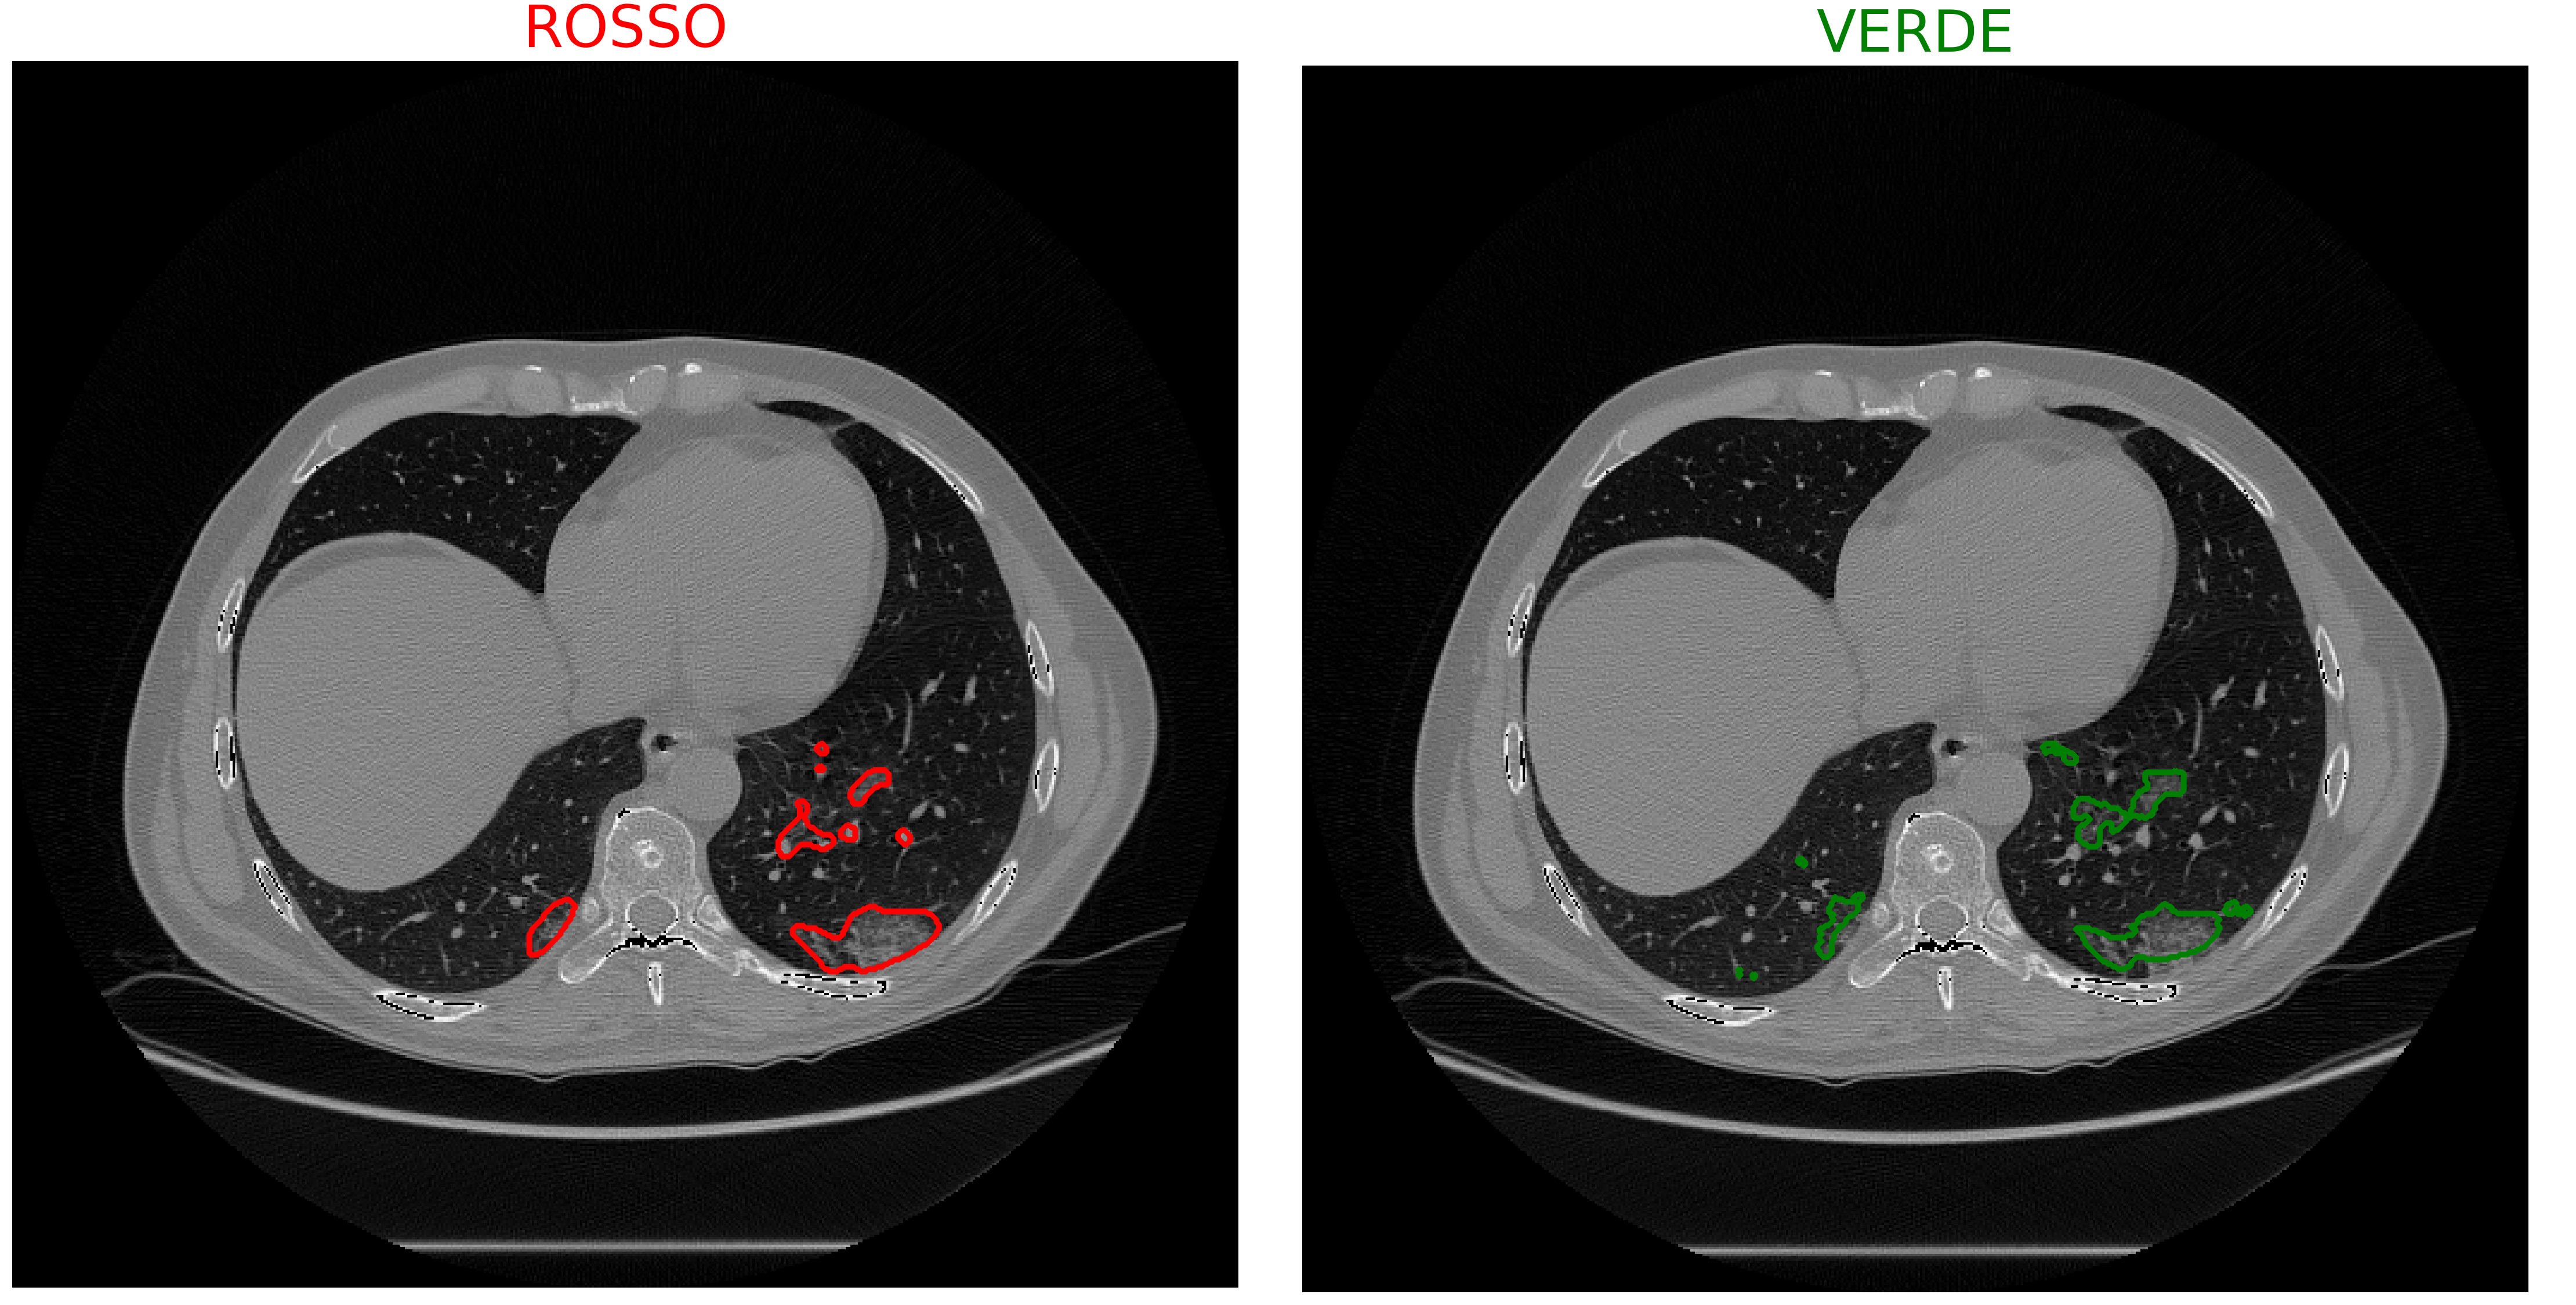
\includegraphics[width=\linewidth]{BlindEval.png}
		\caption{Example of comparison submitted to the experts. The two images report the segmentation of the same slices achieved with two different techniques: Manual and pipeline. Was asked to the expert to decide which one is better, without knowing which technique is used to obtain the segmentation.}\label{fig:Blind}
	\end{figure}

	The scans, organized in this way, was submitted to experts, who have been asked to decide for each scan which segmentation is better or if the quality is equal. For each sample, the whole scan was submitted, considering also the slices without lesion. 

	The core of this method is that the experts do not know which scan corresponds to a specific segmentation technique, so this will lead to an ideally unbiased evaluation. To ensure that, the order of segmentation was shuffled between patients. The expert has validated the scans independently, so for each patient, I have at most $3$ different results. 

	\begin{table}[h!]
		\begin{tabular}{|c|c|c|c|c|c|c|c|c|c|c|}
			\hline
			Patient  	& 1  	 & 2  	  & 3  	   & 4    	& 5  	& 6   	 & 7  	  & 8  		& 9  	& 10	 \\ \hline
			Pipeline	& $0.06$ & $0.28$ & $0.06$ & $0.92$ & $0.06$& $0.41$ & $0.13$ & $0.04$  & $0$ 	& $0.35$ \\ 
			Annotation	& $0.60$ & $0.23$ & $0.80$ & $0.00$	& $0.51$& $0.27$ & $0.53$ & $0.01$  & $0.43$& $0.13$ \\ 
			None		& $0.34$ & $0.49$ & $0.14$ & $0.08$ & $0.42$& $0.32$ & $0.34$ & $0.95$	& $0.57$& $0.52$ \\ \hline
		\end{tabular}\caption{Rate of positive evaluation for each class.   }\label{tab:blind}
	\end{table}

	In \tablename\,\ref{tab:blind} I have reported the results of this evaluation. For each patient I have displayed the rate of positive evaluation for the pipeline segmentation and the annotation. Moreover I have also reported the rate of equal evaluation (None). Notice that this analysis takes into account also the slices in which there aren't lesions. In this way also, the false positives were takes into account. 

	As we can see the pipeline seems to return a better segmentation in more or less a half of the total cases. We have to point out that a  segmentation does not mean the achievement of an inconsistent segmentation, but only that one segmentation is more accurate. 
	
	\begin{figure}
		\centering
		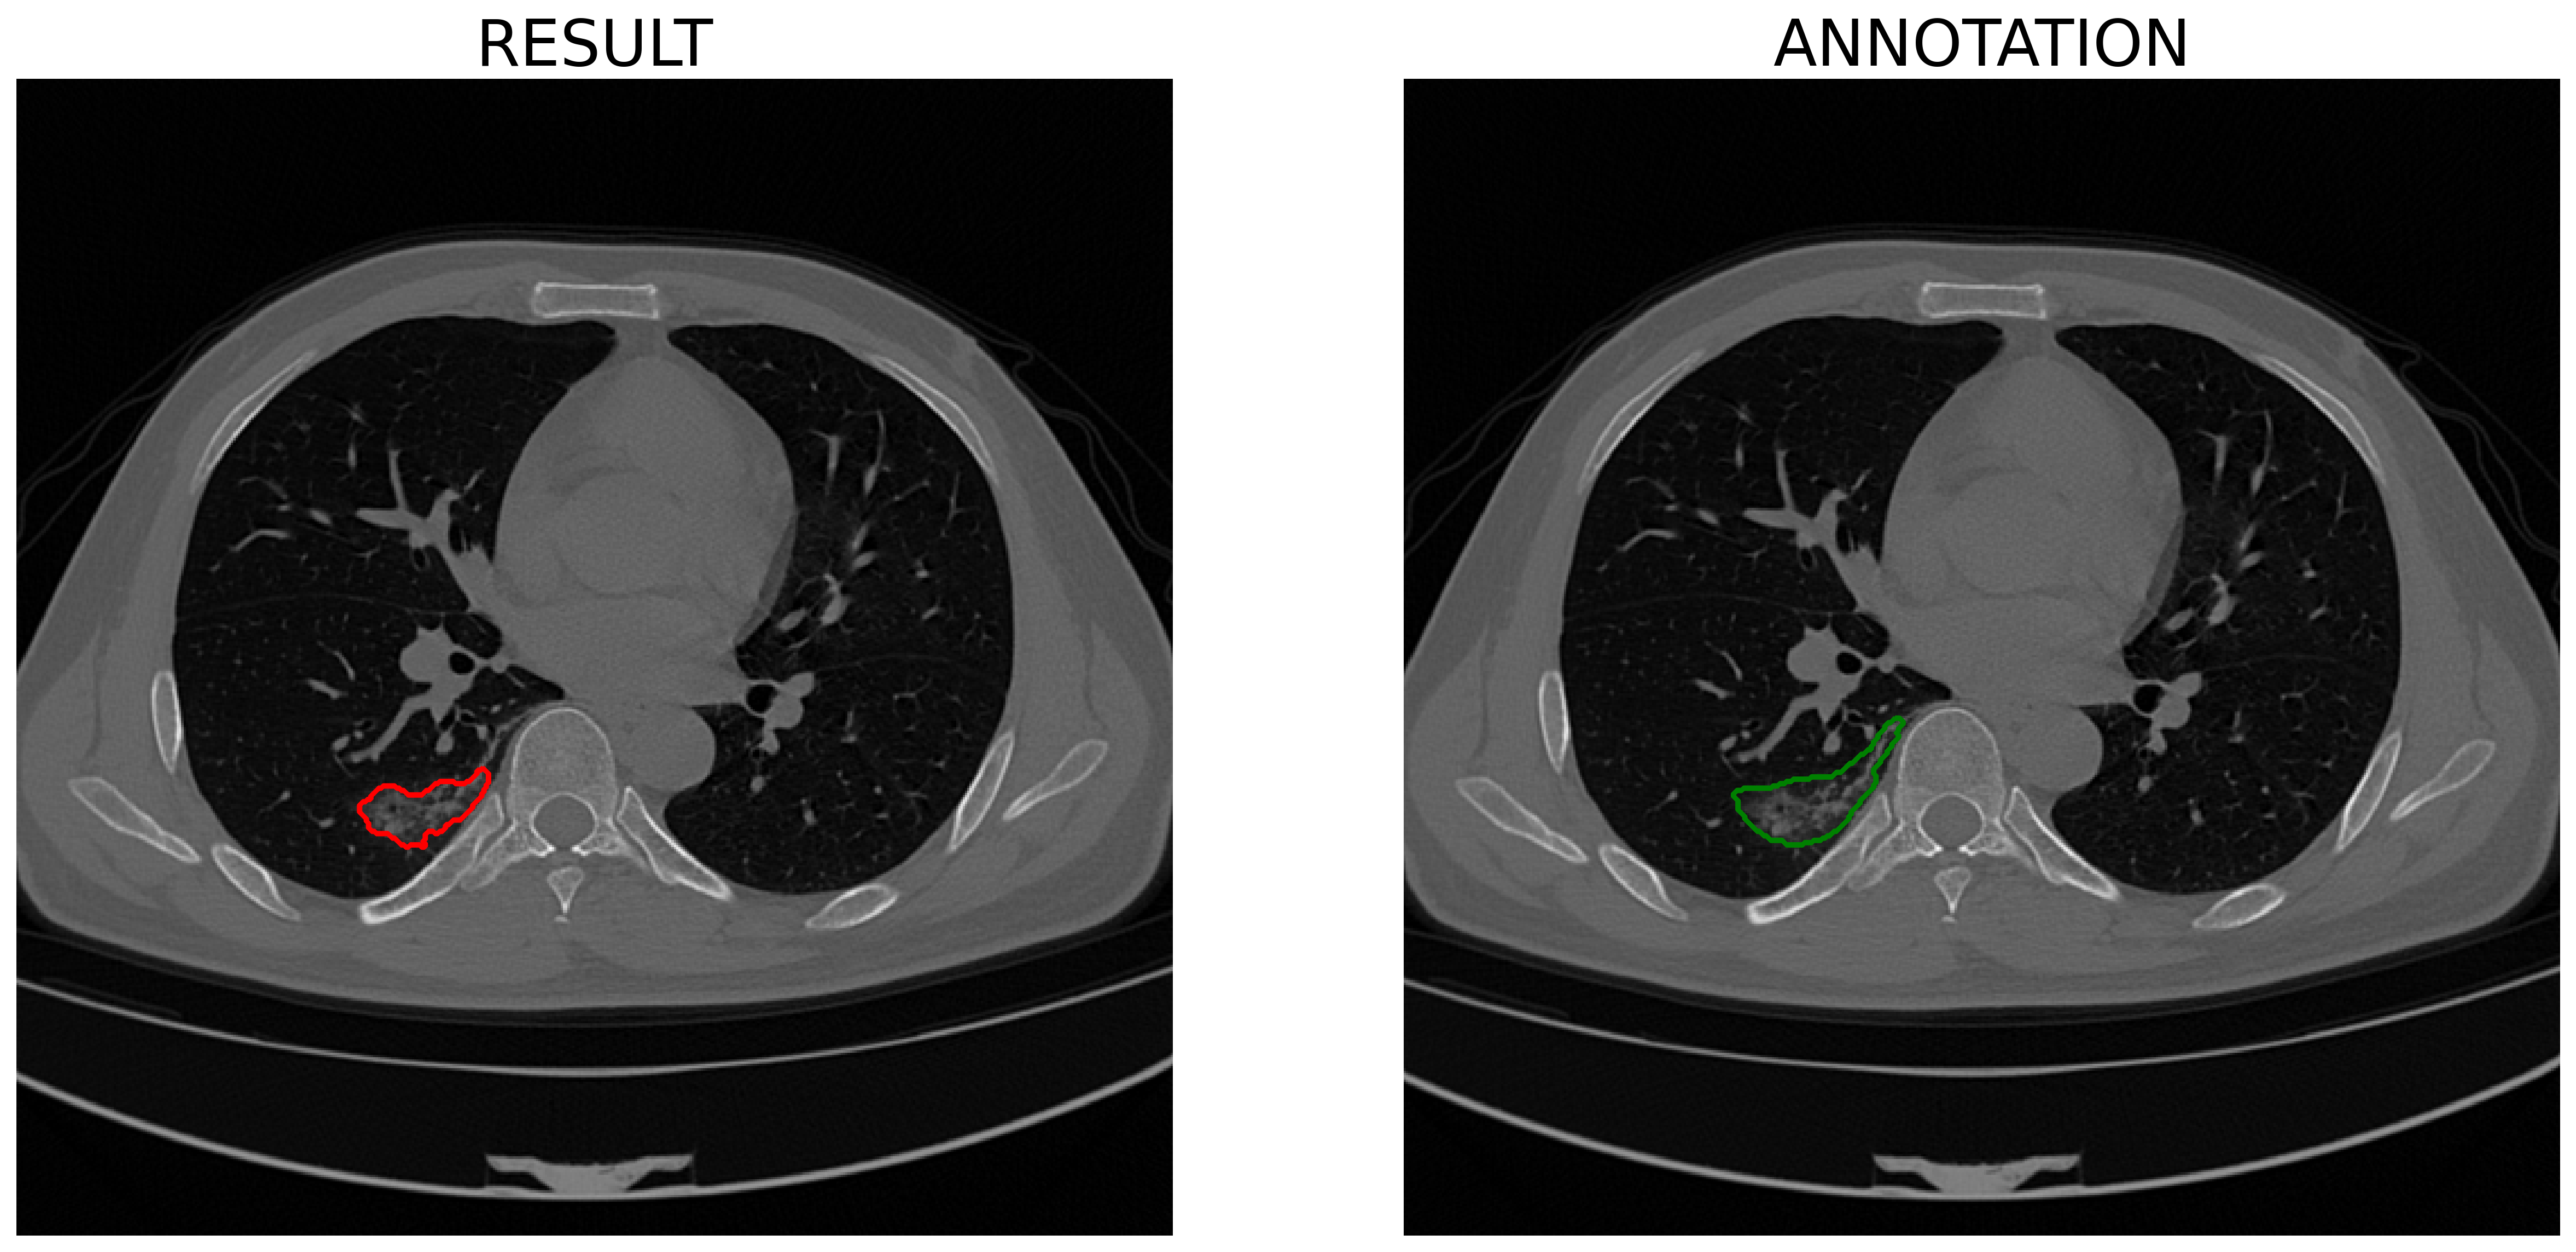
\includegraphics[width=\linewidth]{Patient9.png}
		\caption{Pipeline results vs Manual annotation for the $9_{th}$ patient. As we can see, even if the manual segmentation were classified abetter thatn the pipline one, the last seems to be consistent.}\label{fig:Patient9}
	\end{figure}

	In \figurename\,\ref{fig:Patient9} I have reported a matching between the pipeline segmentation (red) and the manual annotation. As we can see the two results are consistent. However, the pipeline tends to underestimate the lesion area. 
	
	\begin{figure}
		\centering
		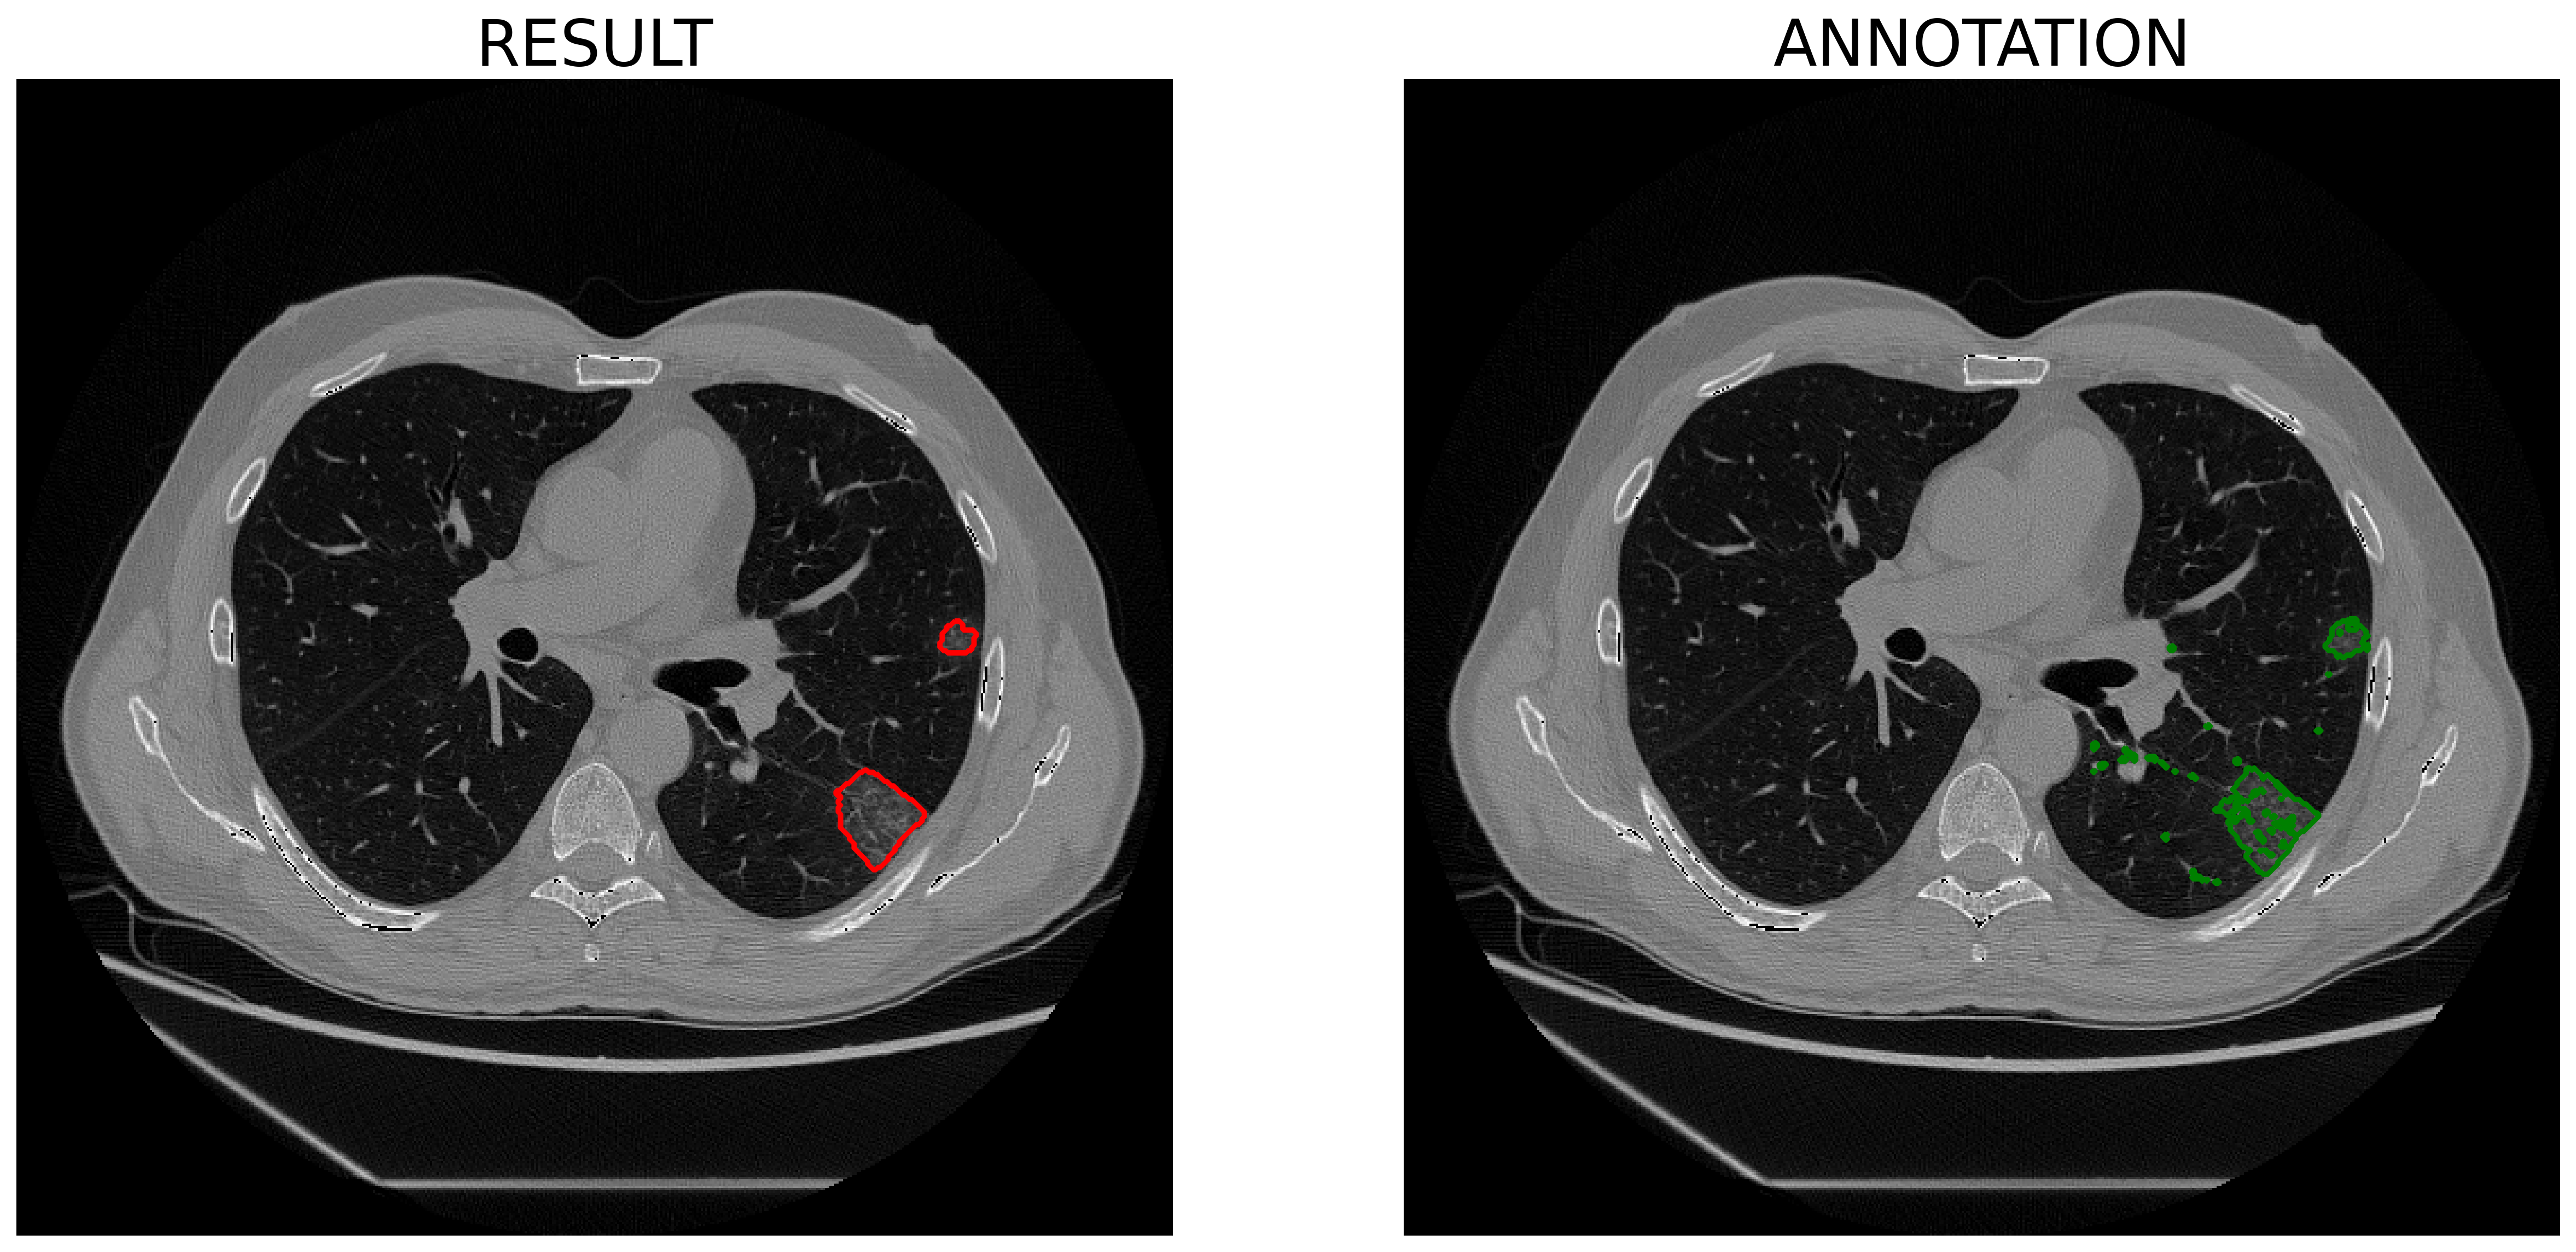
\includegraphics[width=\linewidth]{Patient10.png}
		\caption{Pipeline results vs Manual annotation for the $10_{th}$ patient. As we can see, even if the manual segmentation were classified abetter thatn the pipline one, the last seems to be consistent. We can notice that the oparator has selected also healthy tissues as GGO. }\label{fig:Patient10}
	\end{figure}
	
	In \figurename\,\ref{fig:Patient10} I have matching the segmentation results for patient $10$. The pipeline (red) has evaluated to provide a better lesion identification than the annotation (green). We can notice that in this case some healthy regions are misclassified by the operator, that are correctly removed by the pipeline.
	
	Moreover, we can point out that, at least in the most typical cases, the difference between the pipeline segmentation and annotation is due mainly on the second one, since the subjectivity to the operator experience and the available segmentation time (hour or days) affect the quality. On the other hand, the developed approach does not suffer from these drawbacks, since it is automatic and fast. 
	
	\begin{table}[h!]
		\centering
		\begin{tabular}{|c|c|}
			\hline
			Class 		& Score rate \\ \hline
			Pipeline 	& 0.31		 \\ \hline
			Annotation  & 0.33		 \\ \hline
			None 		& 0.35		 \\ \hline
		\end{tabular}
	\caption{Score rate of positive evaluation for each class. As we can see the results seems to be uniformly distributed.}\label{tab:Rate}
	\end{table}
	
	In the end, as a final consideration, I have measured the rate of positive evaluation for each class, considering all the results provided. The results are reported in \tablename\,\ref{tab:Rate} from we can notice that the pipeline and annotation give positives results more or less with the same rate. Given two different labels it usually it is difficult to spot which is obtained by the pipeline and which belong to an annotation.
	
\end{document}